\section{Guida al codice sviluppato}
\begin{frame}{File modifica e file nuovi}
  \begin{columns}
    \begin{column}{0.7\textwidth}
      Per implementare la \alert{nuova} procedura di autoranging
      è stato necessario intervenire sul codice.\\
      In \textcolor{red}{rosso} sono indicati i file modificati e in
      \textcolor{violet}{viola} i nuovi file prodotti.
    \end{column}
    \begin{column}{0.3\textwidth}
      \centering
      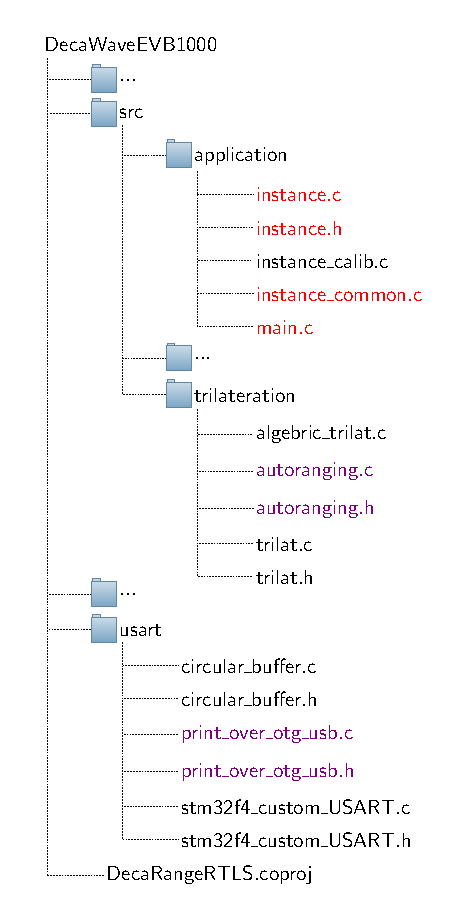
\includegraphics[height=20em]{file_tree.pdf}
    \end{column}
  \end{columns}

\end{frame}
